
%% stripped down version of "bare_jrnl.tex" for use in Casey's Circuits I class.
%% Original version has very good comments for use. You should check it out at
%% http://www.ieee.org/publications_standards/publications/authors/authors_journals.html
%% I run GNU/Linux so I downloaded the "Unix LaTeX2e Transactions Style File" package
%% and based my work off of the sample tex file named "bare_jrnl.tex".

% original author info below (this guy's a rockstar for making his comments so easy to use :P)
%% 2007/01/11
%% by Michael Shell
%% see http://www.michaelshell.org/
%% for current contact information.

\documentclass[journal,twocolumn]{IEEEtran}
% make sure "IEEEtran.cls" is in the path of the tex file you are working on

%graphics package for adding images
\ifCLASSINFOpdf
  \usepackage[pdftex]{graphicx}
\else
   \usepackage[dvips]{graphicx}
\fi

%math package for math equations
\usepackage[cmex10]{amsmath}

%float package for putting images where I fucking tell them to go
\usepackage{float}

%for putting all figures at the end of the document (useful when 
%they are large and unwieldy)
\usepackage[nomarkers]{endfloat}

%center captions under their images/figures
\usepackage{caption}

%for background color for listings
\usepackage{color}
\definecolor{light-gray}{gray}{0.95}

%for sourcecode
\usepackage{listings}
\lstset{breaklines=true,
language=gnuplot,
basicstyle=\scriptsize,
showspaces=false,
showstringspaces=false,
frame=single,
backgroundcolor=\color{light-gray}}

%For hyperlinks
\usepackage{hyperref}

\begin{document}

% paper title
% can use linebreaks \\ within to get better formatting as desired
\title{Project 3: Collection and Analysis of Wireless Signals}
\author{Preston~Maness}

% header
\markboth{Texas State University, Dr. Hudson, EE4372, Spring 2014}%
{}

% make the title area
\maketitle

% Give the abstract of your lab here
\begin{abstract}
A route around campus was taken on foot in order to sample cell phone, GPS, 
and WiFi signals. An Android smartphone with the RF Signal Tracker 
app was used to sample and store the various data associated with each type 
of wireless signal. Analysis was then performed on signal strength over 
time and location for each type of signal. Additionally, wireless network
SSID and BSSID characteristics were correlated against location on the 
Texas State University San Marcos campus.

\end{abstract}

% Split your lab report into sections by calling \section{Section name}
\section{Sampling Methodology and Route}
\IEEEPARstart{T}{his} project makes use of an app titled ``RF Signal Tracker'' 
by developer Ken Hunt in the Google Play app store for Android smart phones. 
The particular device utilized was a Samsung Galaxy S Relay 4G, model string 
SGH-T699. A path was walked around campus, with this device running this app,
to sample cellular signals, GPS signals, and WiFi signals at regular intervals
and store the results in a CSV file. Analysis was then performed on the data.

The route is detailed in figure~\ref{fig_path} as the red line over the Google
Maps Satellite image. The path started at the RFM building, and ended at the
commuter parking lot near the soccer fields. The entire path was walked at 
approximately the same speed, with only one stop for a traffic light. \emph{
Due to this fact, the relationship between time and location is relatively 
linear with only minor phase shifts.} Given this relationship, the data in 
this report is plotted against time, with the understanding that the position 
of the sampler when $x$ percent of the data has been plotted roughly 
corresponds to $x$ percent of the path having been travelled.

\begin{figure*}
\begin{center}
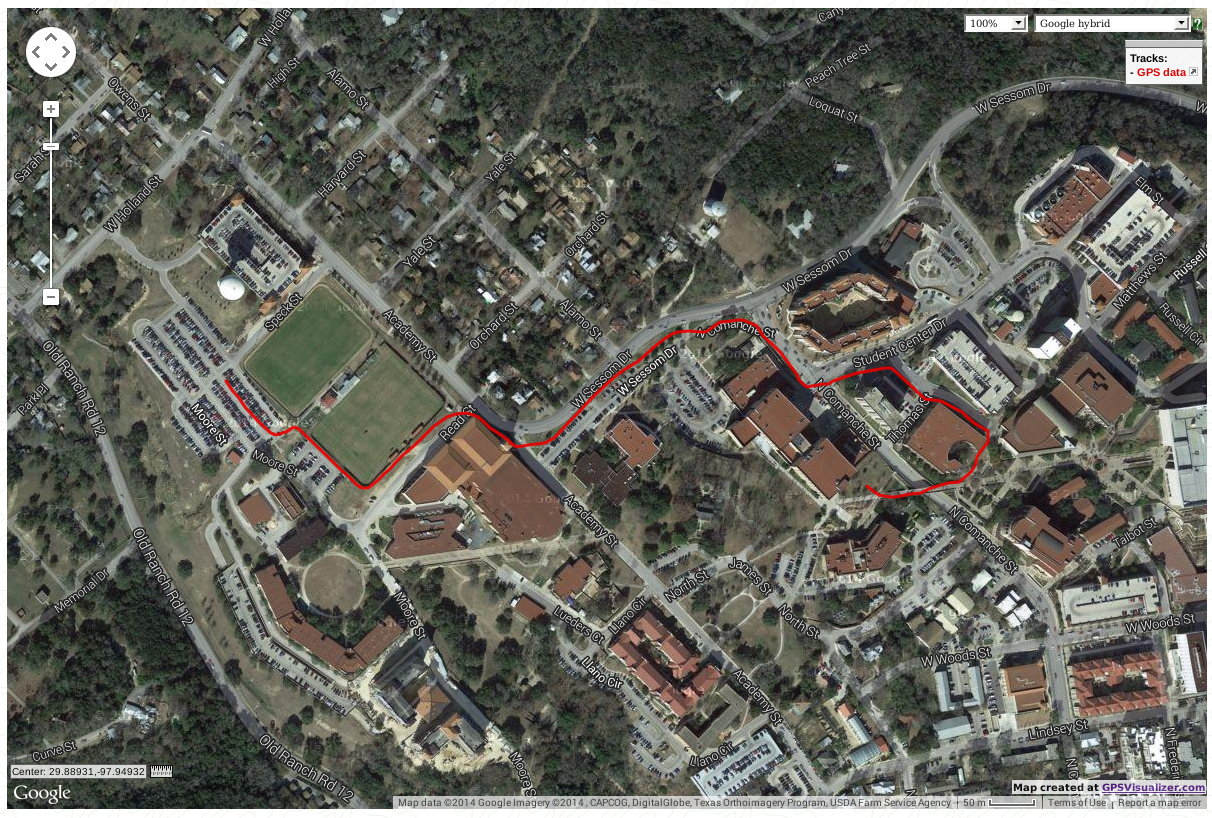
\includegraphics[scale=0.4]{path-data/Path-Taken-Starting-At-Mitte.png}
\caption{Path Taken Around Campus}
\label{fig_path}
\end{center}
\end{figure*}

\section{Data}

The data is kept in two principal csv files on a git repository located at 
the following URLs:

\begin{itemize}
\item
Cell and GPS data: \url{https://raw.githubusercontent.com/aggroskater/ee4372-comm-networks/master/project-3-wireless-signal-sampling/cell-data/export_140321144244.csv}
\item
WiFi data: \url{https://raw.githubusercontent.com/aggroskater/ee4372-comm-networks/master/project-3-wireless-signal-sampling/wifi-data/wifi_140403220558.csv}
\end{itemize}

The data collected Cell and GPS data every 5 to 6 seconds, and WiFi data every 
7 or 8 seconds. It is important to note that it appears as if the sampling 
software was unable to keep up with the polling requests for at least the 
first minute for the WiFi data. There are multiple sets of WiFi data that have
the same timestamp, but different GPS coordinates during this first minute. The
overal trends gleaned from the data, however, do not suffer unnecessarily from
this glitch.

Numerous gnuplot scripts were utilized to plot this data in different ways. 
Along the way, various ``helper'' CSVs were generated to ease plotting with 
gnuplot. These helper CSVs may all be found in the repository, as can  the 
gnuplot scripts. The main url for the repository is below:

\begin{itemize}
\item
\url{https://github.com/aggroskater/ee4372-comm-networks/tree/master/project-3-wireless-signal-sampling}
\end{itemize}

\section{Cellular Data Analysis}

The Received Signal Strength Indication (RSSI, units dBm) of the cellular 
signal was plotted over time, as was the class of signal (regular 2G vs data 
3G/4G). The results can be found in figure~\ref{fig_cell_1}. It can be seen 
that the signal strength correlates with the presence of buildings: the more 
buildings there are, the lower the signal strength tends to be.

\begin{figure*}
\begin{center}
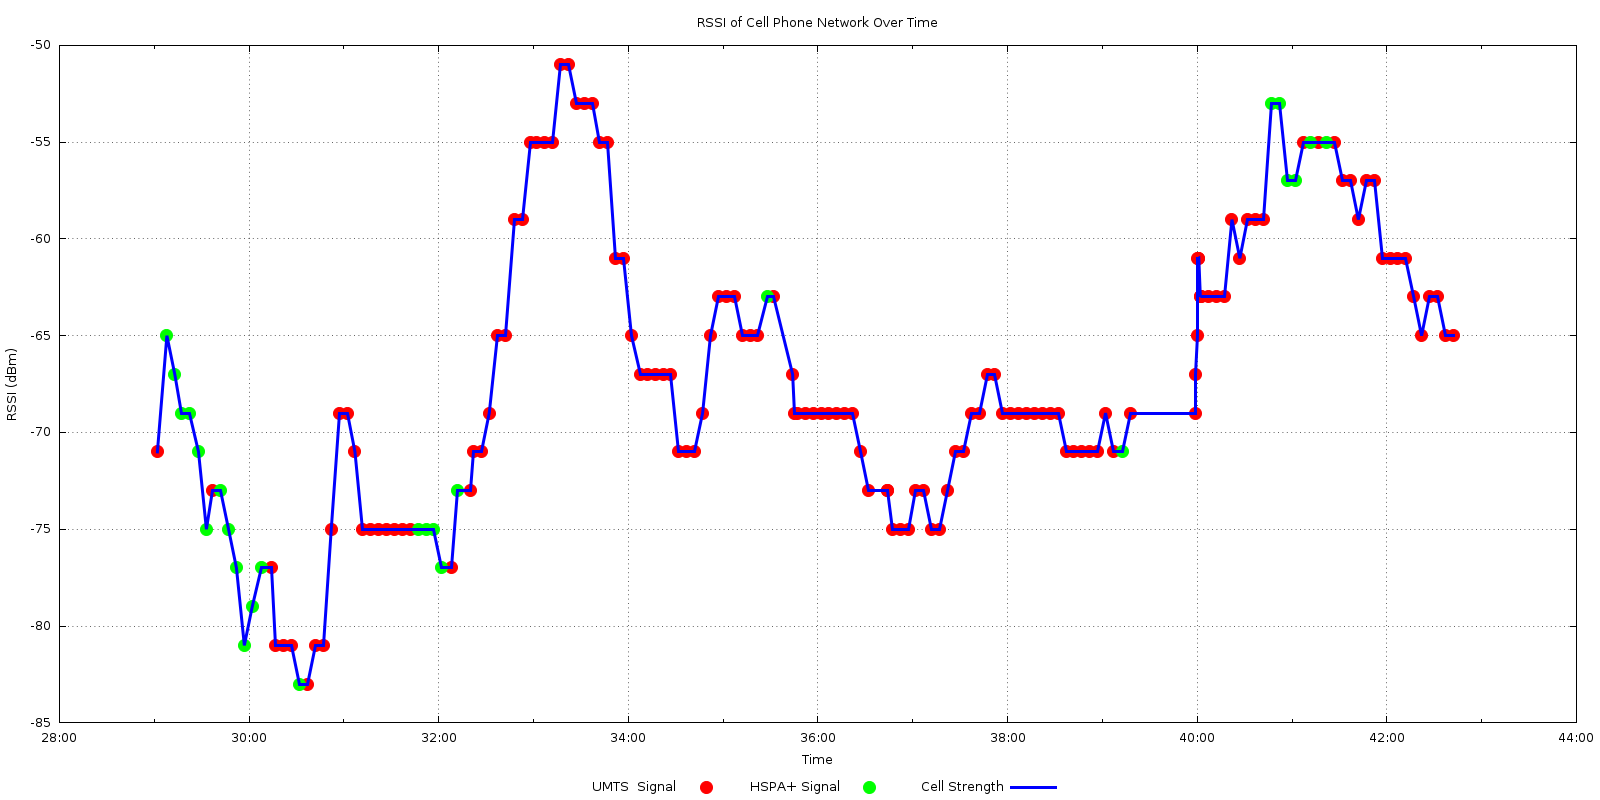
\includegraphics[scale=0.3]{cell-data/cell.png}
\caption{RSSI of Cellular Signal Over Time}
\label{fig_cell_1}
\end{center}
\end{figure*}

As well, mobile data transfer over time was also plotted in
figure~\ref{fig_cell_2}. In particular, take note that mobile data transfer
only occured when there was an HSPA+ (3G/4G) signal to the cellular handset.
Throughput of the data connection was not investigated for this report.

\begin{figure*}
\begin{center}
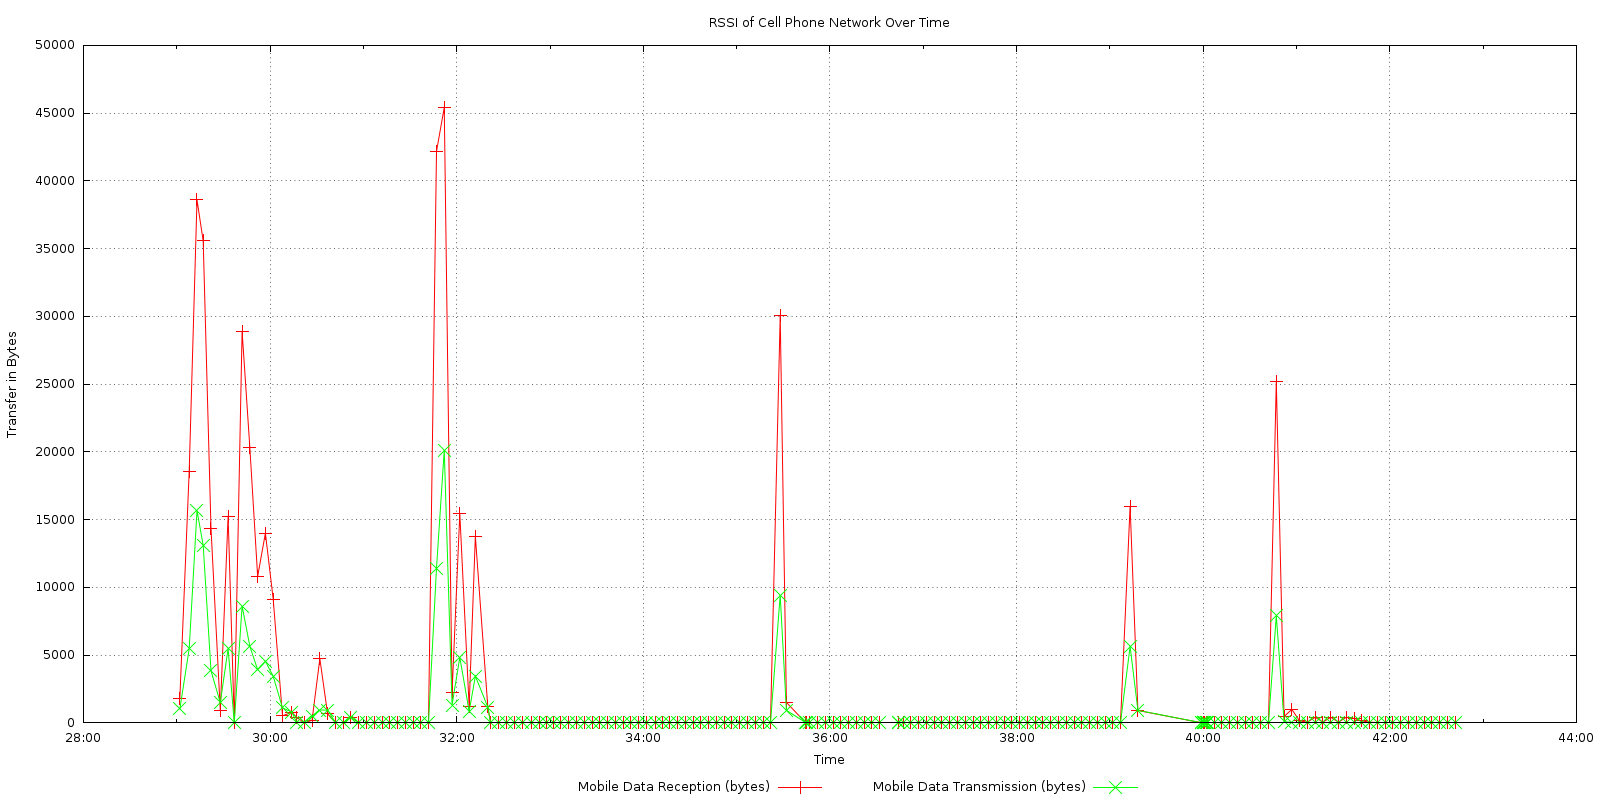
\includegraphics[scale=0.3]{cell-data/cell-2.png}
\caption{Mobile Data Transfer Over Time}
\label{fig_cell_2}
\end{center}
\end{figure*}

The code for these plots can be found in the repo mentioned in the Data 
section of this report.

\section{WiFi Data Analysis}

A first impression of the WiFi data leads to the conclusion that the 
WiFi spectrum is quite crowded around Texas State. Figure~\ref{fig_wifi_1}
showcases over 100 unique SSIDs that were sampled on the route. 65 of these 
were ``unknown'' signals that were broadcasting a BSSID on the WiFi spectrum, 
but did not supply SSIDs. It is suspected that these were WiFi signals 
from personal devices such as mobile phones and laptops that were not acting 
as access points.

\begin{figure*}
\begin{center}
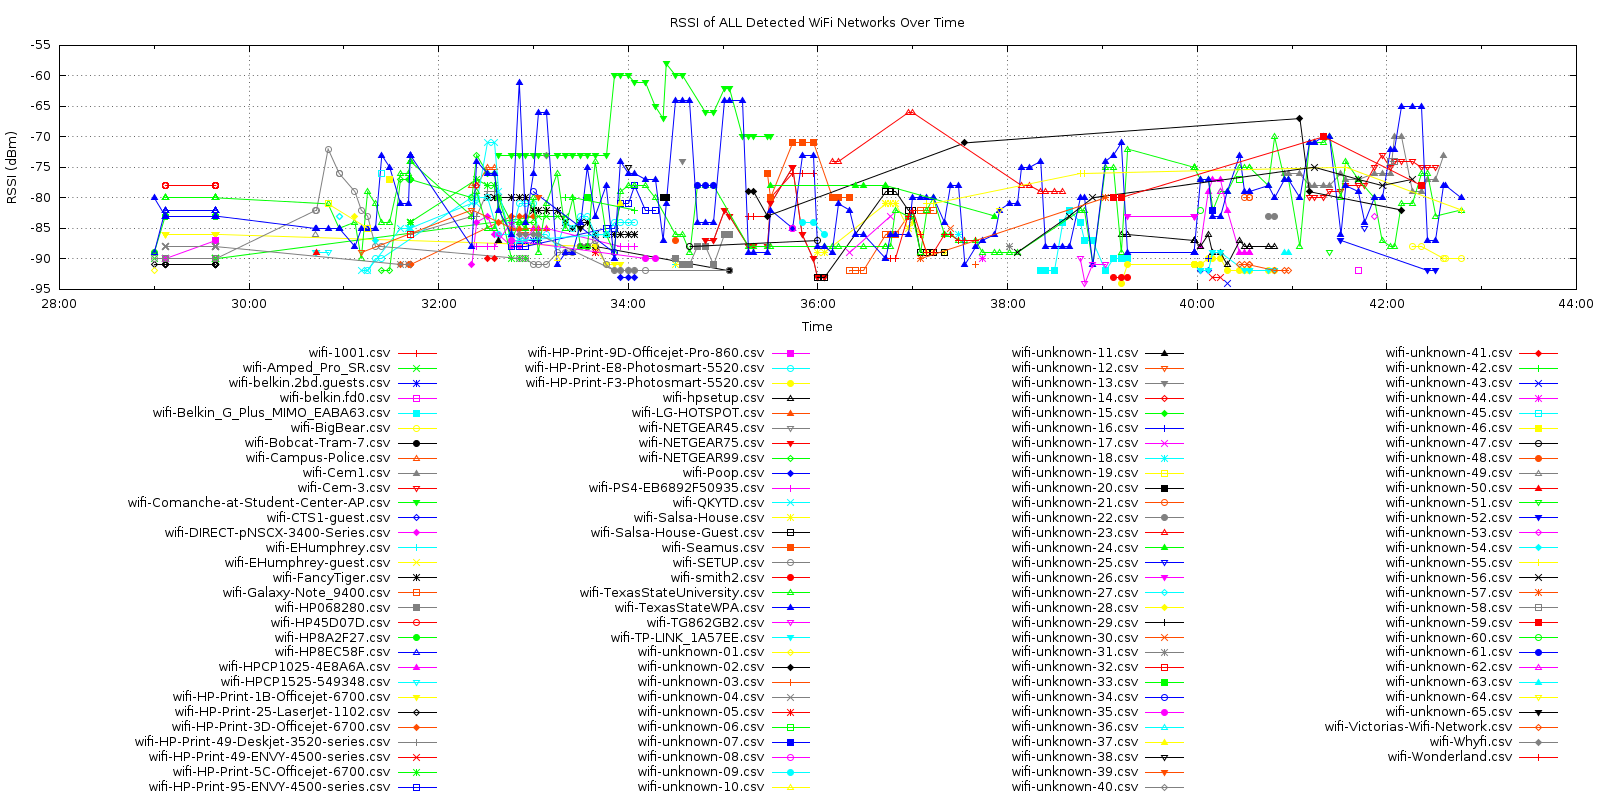
\includegraphics[scale=0.3]{wifi-data/001-everything.png}
\caption{ALL WiFi SSIDs}
\label{fig_wifi_1}
\end{center}
\end{figure*}

Eliminating the unknowns from the plot, as in Figure~\ref{fig_wifi_2}, still
shows a relatively crowded spectrum, but more trends are evident without the
noise of the uknowns. The solid blue triangle line in particular is the
``TexasStateWPA'' SSID that most students, faculty, and other staff utilize to
connect to the Texas State network. Between the 30 minute and 32 minute marks,
there is relatively little SSID detection. This corresponds to the walk away
from RFM, over the bridge, and toward the main campus. From the 32 minute to 
37 minute marks, there is more SSID detection that corresponds with the 
Nursing and Student Center buildings, followed by several dorm rooms. From the
37 minute to 39 minute mark, the walk along Sessom Drive toward the Rec center
has lower SSID detection. Upon walking along the Rec Center and toward the 
athletic dorms, SSID detection rises again until the sampler reaches the 
parking lot.

\begin{figure*}
\begin{center}
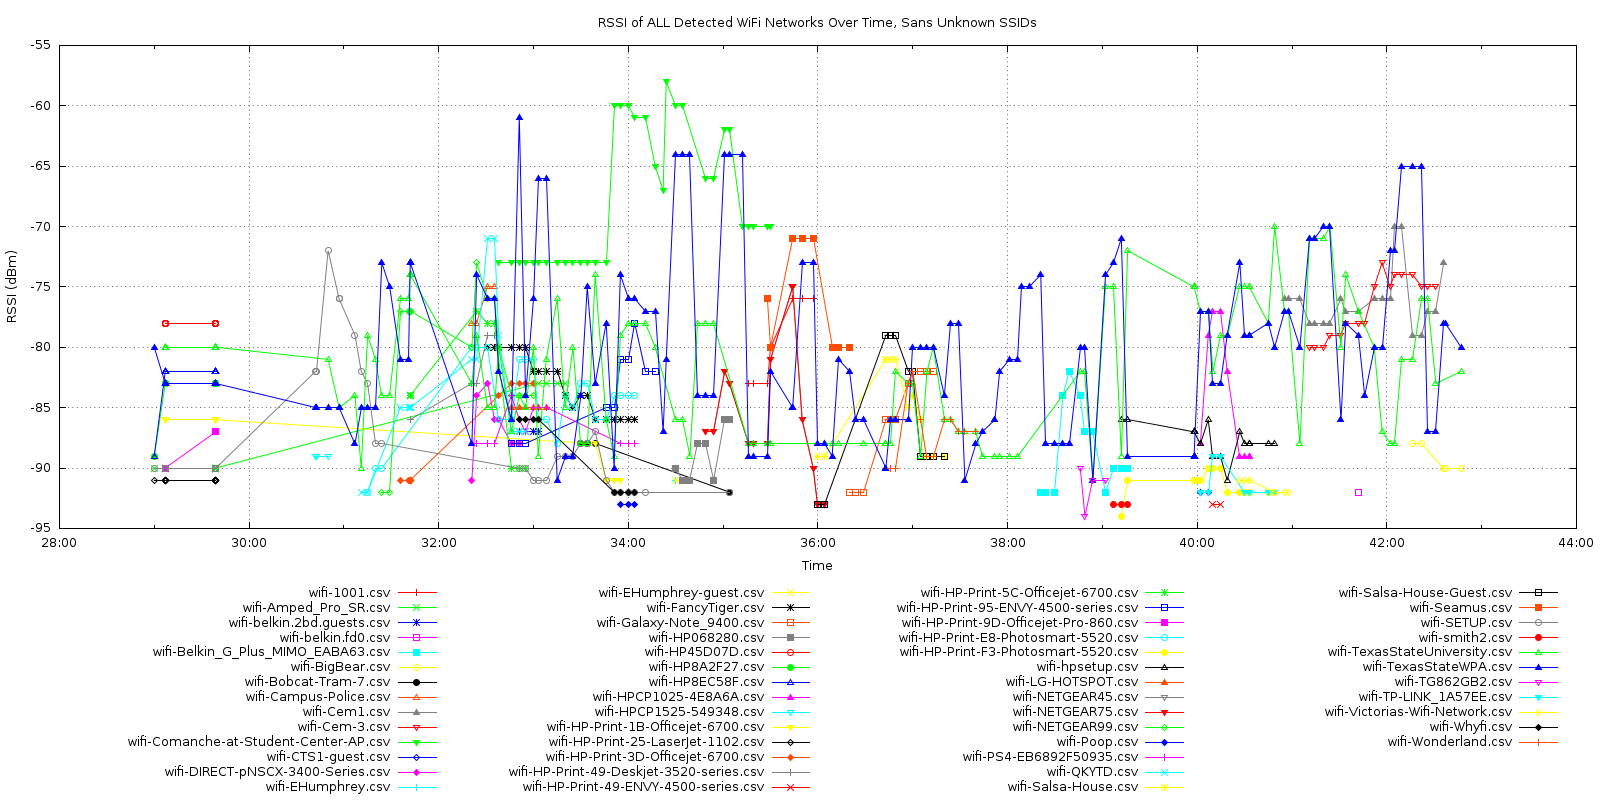
\includegraphics[scale=0.3]{wifi-data/002-all-but-unknowns.png}
\caption{All WiFi SSIDs Except Unknowns}
\label{fig_wifi_2}
\end{center}
\end{figure*}

The TexasStateWPA and TexasStateUniversity networks are plotted in 
Figure~\ref{fig_wifi_3}. Not revealed by the plot, however, is that this 
WiFi network is supplied by numerous independent devices. As the sampler 
walks out of range of one access point, the connection gets handed off to 
another access point. This is evident in the logs, as the SSID stays the 
same --TexasStateWPA-- while the BSSID that identifies the unique hardware 
supply the SSID changes.

\begin{figure*}
\begin{center}
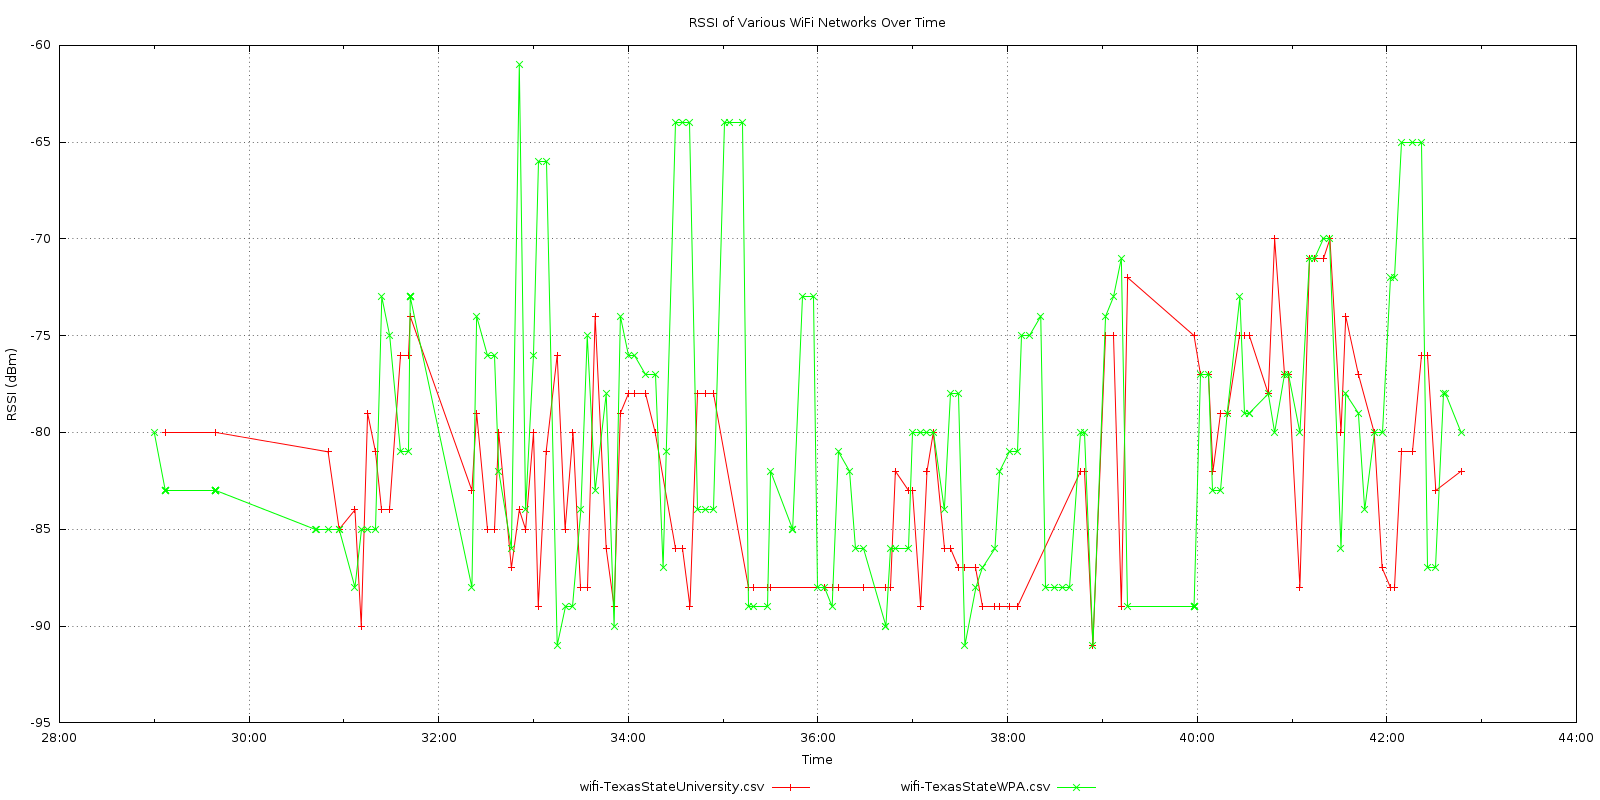
\includegraphics[scale=0.3]{wifi-data/003-texas-state-wireless.png}
\caption{Texas State Wireless Network (TexasStateWPA and TexasStateUniversity)}
\label{fig_wifi_3}
\end{center}
\end{figure*}

Figure~\ref{fig_wifi_4} is provided to illustrate the presence of two other 
``official'' Texas State wireless SSIDs. The ``Comanche at Student Center'' 
SSID is found near the student center between the 33 and 35 minute marks. 
During this particular segment of the path, the SSID of a Bobcat Tram 
was also briefly detected (two samples): ``BobcatTram7''. It is suspected that
this signal was associated with a moving Bobcat Tram as it either arrived or 
departed from the Student Center pick-up/drop-off zone.

\begin{figure*}
\begin{center}
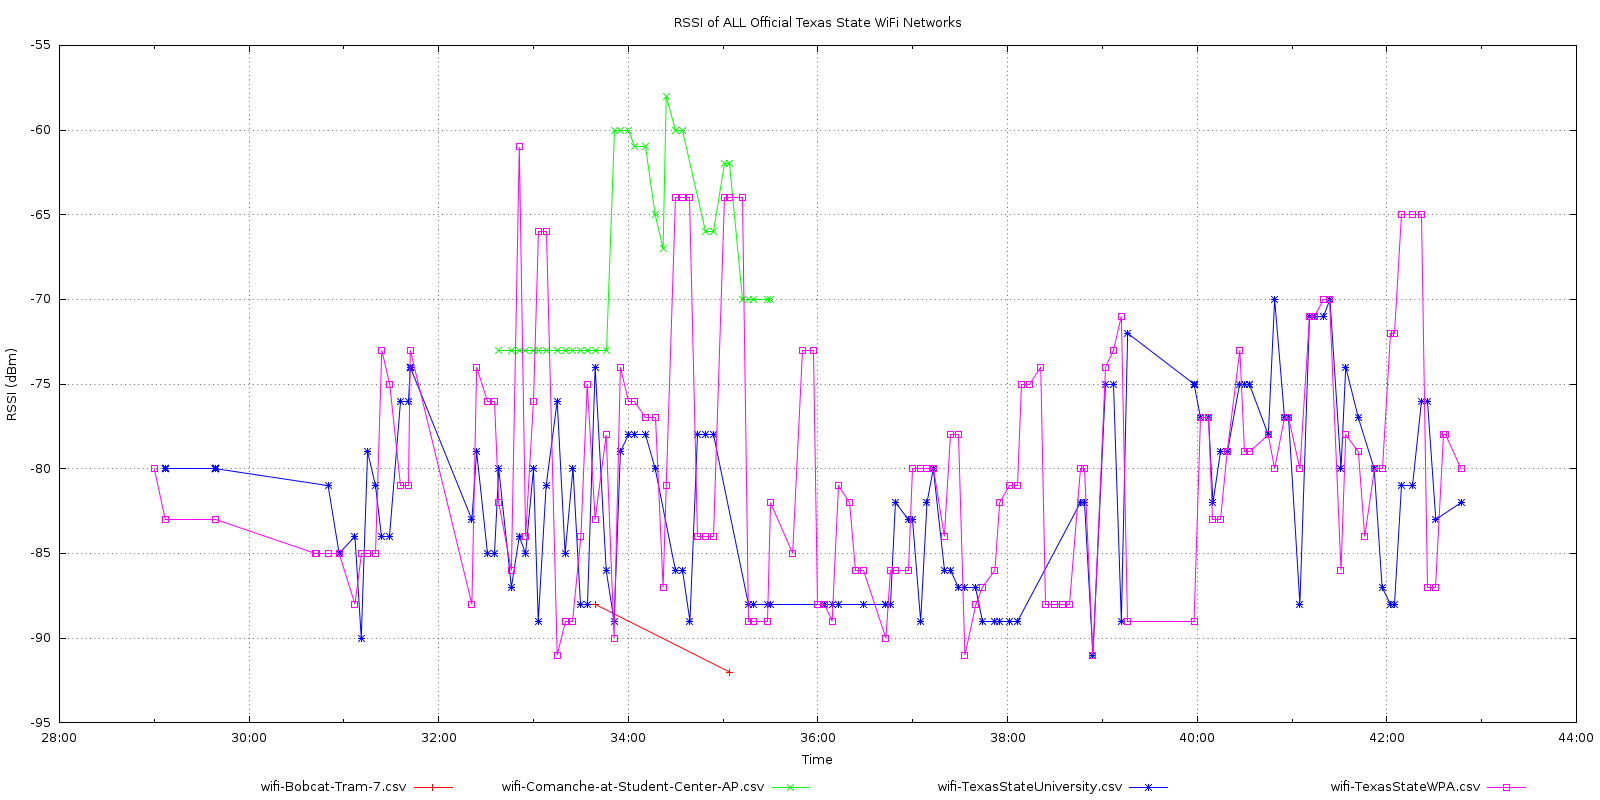
\includegraphics[scale=0.3]{wifi-data/004-official-txstate.png}
\caption{All ``official'' Texas State Wireless SSIDs}
\label{fig_wifi_4}
\end{center}
\end{figure*}

Figure~\ref{fig_wifi_5} shows the signal strength of various SSIDs associated 
with HP printing devices. Three distinct clusters are evident. The first is 
around the 29 minute mark. Numerous HP printing devices are detected and are 
likely originated in the RFM building. Crossing the bridge, many more printing 
devices are detected, presumably from the Nursing and Student Center buildings 
as well as the nearby dorm rooms. These types of SSIDs drop off afterward 
until the sampler nears the athletic dorms near the rec center and commuter 
parking lot, where some brief SSID detection again occurs.

\begin{figure*}
\begin{center}
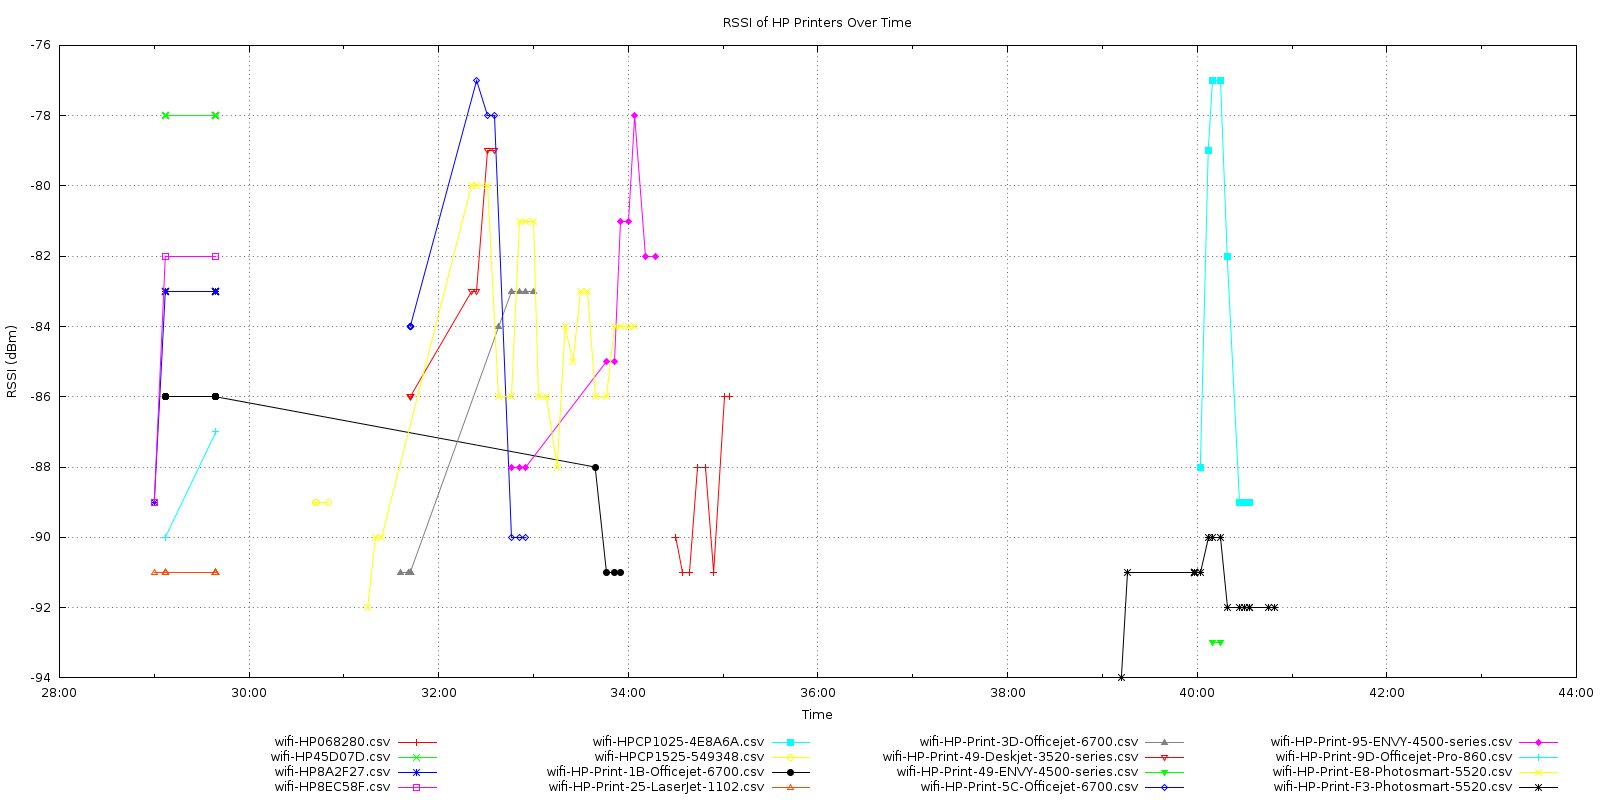
\includegraphics[scale=0.3]{wifi-data/005-printers.png}
\caption{WiFi Printing Devices}
\label{fig_wifi_5}
\end{center}
\end{figure*}

Finally, Figure~\ref{fig_wifi_6} plots the unknown WiFi signals by themselves. 
They appear to occur relatively uniformly throughout the sampling path. It is 
suspected that these correspond to WiFi clients, rather than access points.

\begin{figure*}
\begin{center}
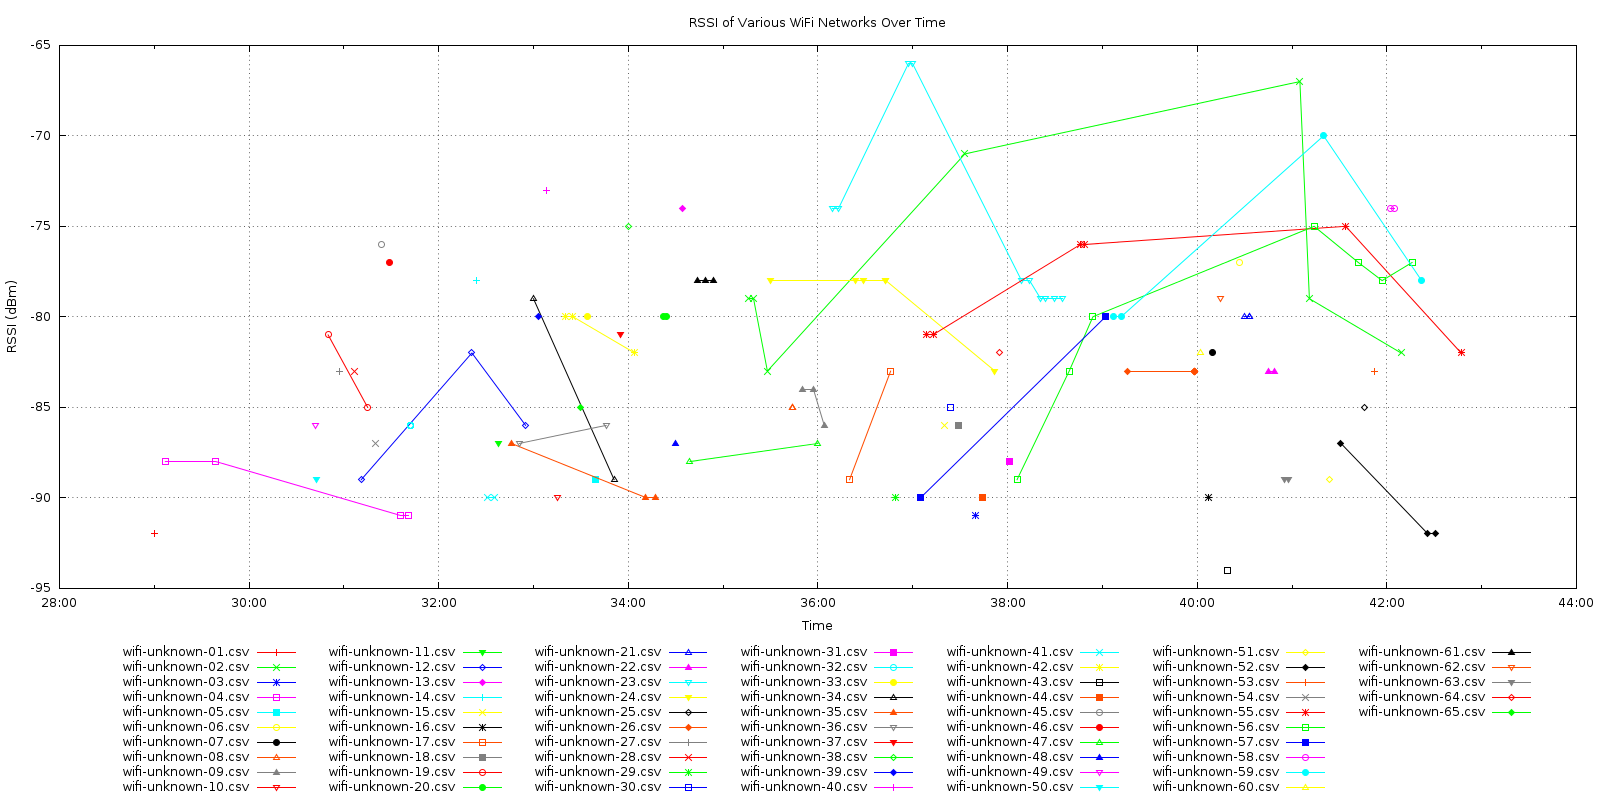
\includegraphics[scale=0.3]{wifi-data/006-unknowns.png}
\caption{WiFi Signals With No SSID (Unknowns)}
\label{fig_wifi_6}
\end{center}
\end{figure*}

\section{Conclusion}

Lol conclusions are cool.

%\appendix[Gnuplot Scripts]

%This appendix holds numerous gnuplot scripts utilized in the 
%generation of the plots found in this report. Comments were used 
%to run different instances of the plot with different data by 
%commenting out every line that was not to be plotted for any 
%given run (hacky, sure, but I've got five other classes to deal 
%with). This code can be found in a more digitally accesible manner 
%at the github repo located at \url{https://github.com/aggroskater/ee4372-comm-networks/tree/master/project-3-wireless-signal-sampling}.

%\lstinputlisting[
%caption={Cellular Data Plotting},
%label={lst-cell} 
%]{cell-data/cell.plt}

%\lstinputlisting[
%caption={WiFi Data Plotting},
%label={lst-wifi}
%]{wifi-data/wifi.plt}

\end{document}
